\documentclass[1p]{elsarticle_modified}
%\bibliographystyle{elsarticle-num}

%\usepackage[colorlinks]{hyperref}
%\usepackage{abbrmath_seonhwa} %\Abb, \Ascr, \Acal ,\Abf, \Afrak
\usepackage{amsfonts}
\usepackage{amssymb}
\usepackage{amsmath}
\usepackage{amsthm}
\usepackage{scalefnt}
\usepackage{amsbsy}
\usepackage{kotex}
\usepackage{caption}
\usepackage{subfig}
\usepackage{color}
\usepackage{graphicx}
\usepackage{xcolor} %% white, black, red, green, blue, cyan, magenta, yellow
\usepackage{float}
\usepackage{setspace}
\usepackage{hyperref}

\usepackage{tikz}
\usetikzlibrary{arrows}

\usepackage{multirow}
\usepackage{array} % fixed length table
\usepackage{hhline}

%%%%%%%%%%%%%%%%%%%%%
\makeatletter
\renewcommand*\env@matrix[1][\arraystretch]{%
	\edef\arraystretch{#1}%
	\hskip -\arraycolsep
	\let\@ifnextchar\new@ifnextchar
	\array{*\c@MaxMatrixCols c}}
\makeatother %https://tex.stackexchange.com/questions/14071/how-can-i-increase-the-line-spacing-in-a-matrix
%%%%%%%%%%%%%%%

\usepackage[normalem]{ulem}

\newcommand{\msout}[1]{\ifmmode\text{\sout{\ensuremath{#1}}}\else\sout{#1}\fi}
%SOURCE: \msout is \stkout macro in https://tex.stackexchange.com/questions/20609/strikeout-in-math-mode

\newcommand{\cancel}[1]{
	\ifmmode
	{\color{red}\msout{#1}}
	\else
	{\color{red}\sout{#1}}
	\fi
}

\newcommand{\add}[1]{
	{\color{blue}\uwave{#1}}
}

\newcommand{\replace}[2]{
	\ifmmode
	{\color{red}\msout{#1}}{\color{blue}\uwave{#2}}
	\else
	{\color{red}\sout{#1}}{\color{blue}\uwave{#2}}
	\fi
}

\newcommand{\Sol}{\mathcal{S}} %segment
\newcommand{\D}{D} %diagram
\newcommand{\A}{\mathcal{A}} %arc


%%%%%%%%%%%%%%%%%%%%%%%%%%%%%5 test

\def\sl{\operatorname{\textup{SL}}(2,\Cbb)}
\def\psl{\operatorname{\textup{PSL}}(2,\Cbb)}
\def\quan{\mkern 1mu \triangleright \mkern 1mu}

\theoremstyle{definition}
\newtheorem{thm}{Theorem}[section]
\newtheorem{prop}[thm]{Proposition}
\newtheorem{lem}[thm]{Lemma}
\newtheorem{ques}[thm]{Question}
\newtheorem{cor}[thm]{Corollary}
\newtheorem{defn}[thm]{Definition}
\newtheorem{exam}[thm]{Example}
\newtheorem{rmk}[thm]{Remark}
\newtheorem{alg}[thm]{Algorithm}

\newcommand{\I}{\sqrt{-1}}
\begin{document}

%\begin{frontmatter}
%
%\title{Boundary parabolic representations of knots up to 8 crossings}
%
%%% Group authors per affiliation:
%\author{Yunhi Cho} 
%\address{Department of Mathematics, University of Seoul, Seoul, Korea}
%\ead{yhcho@uos.ac.kr}
%
%
%\author{Seonhwa Kim} %\fnref{s_kim}}
%\address{Center for Geometry and Physics, Institute for Basic Science, Pohang, 37673, Korea}
%\ead{ryeona17@ibs.re.kr}
%
%\author{Hyuk Kim}
%\address{Department of Mathematical Sciences, Seoul National University, Seoul 08826, Korea}
%\ead{hyukkim@snu.ac.kr}
%
%\author{Seokbeom Yoon}
%\address{Department of Mathematical Sciences, Seoul National University, Seoul, 08826,  Korea}
%\ead{sbyoon15@snu.ac.kr}
%
%\begin{abstract}
%We find all boundary parabolic representation of knots up to 8 crossings.
%
%\end{abstract}
%\begin{keyword}
%    \MSC[2010] 57M25 
%\end{keyword}
%
%\end{frontmatter}

%\linenumbers
%\tableofcontents
%
\newcommand\colored[1]{\textcolor{white}{\rule[-0.35ex]{0.8em}{1.4ex}}\kern-0.8em\color{red} #1}%
%\newcommand\colored[1]{\textcolor{white}{ #1}\kern-2.17ex	\textcolor{white}{ #1}\kern-1.81ex	\textcolor{white}{ #1}\kern-2.15ex\color{red}#1	}

{\Large $\underline{12n_{0588}~(K12n_{0588})}$}

\setlength{\tabcolsep}{10pt}
\renewcommand{\arraystretch}{1.6}
\vspace{1cm}\begin{tabular}{m{100pt}>{\centering\arraybackslash}m{274pt}}
\multirow{5}{120pt}{
	\centering
	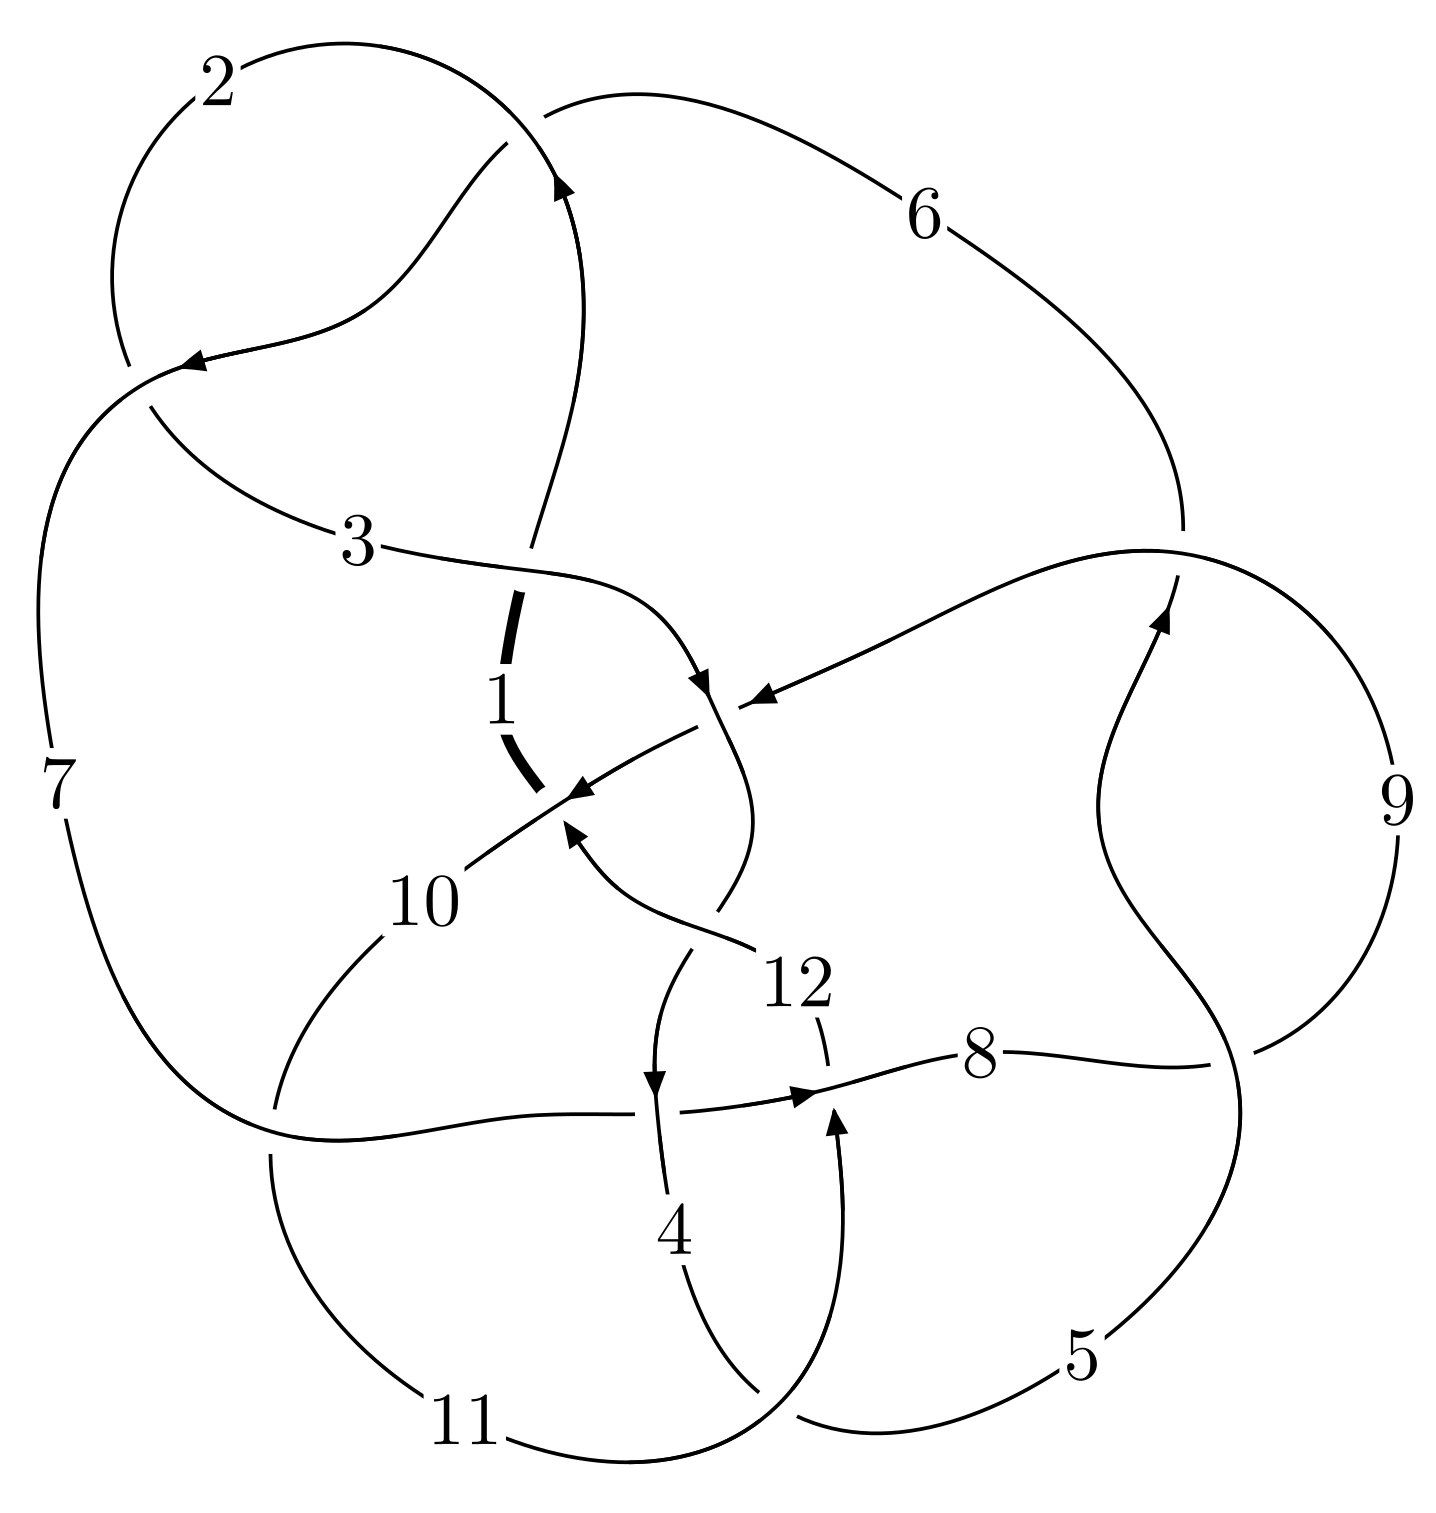
\includegraphics[width=112pt]{../../../GIT/diagram.site/Diagrams/png/2677_12n_0588.png}\\
\ \ \ A knot diagram\footnotemark}&
\allowdisplaybreaks
\textbf{Linearized knot diagam} \\
\cline{2-2}
 &
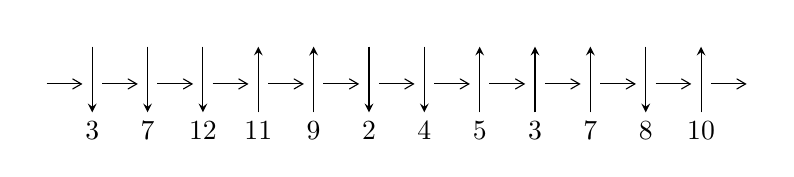
\begin{tikzpicture}[x=20pt, y=17pt]
	% nodes
	\node (C0) at (0, 0) {};
	\node (C1) at (1, 0) {};
	\node (C1U) at (1, +1) {};
	\node (C1D) at (1, -1) {3};

	\node (C2) at (2, 0) {};
	\node (C2U) at (2, +1) {};
	\node (C2D) at (2, -1) {7};

	\node (C3) at (3, 0) {};
	\node (C3U) at (3, +1) {};
	\node (C3D) at (3, -1) {12};

	\node (C4) at (4, 0) {};
	\node (C4U) at (4, +1) {};
	\node (C4D) at (4, -1) {11};

	\node (C5) at (5, 0) {};
	\node (C5U) at (5, +1) {};
	\node (C5D) at (5, -1) {9};

	\node (C6) at (6, 0) {};
	\node (C6U) at (6, +1) {};
	\node (C6D) at (6, -1) {2};

	\node (C7) at (7, 0) {};
	\node (C7U) at (7, +1) {};
	\node (C7D) at (7, -1) {4};

	\node (C8) at (8, 0) {};
	\node (C8U) at (8, +1) {};
	\node (C8D) at (8, -1) {5};

	\node (C9) at (9, 0) {};
	\node (C9U) at (9, +1) {};
	\node (C9D) at (9, -1) {3};

	\node (C10) at (10, 0) {};
	\node (C10U) at (10, +1) {};
	\node (C10D) at (10, -1) {7};

	\node (C11) at (11, 0) {};
	\node (C11U) at (11, +1) {};
	\node (C11D) at (11, -1) {8};

	\node (C12) at (12, 0) {};
	\node (C12U) at (12, +1) {};
	\node (C12D) at (12, -1) {10};
	\node (C13) at (13, 0) {};

	% arrows
	\draw[->,>={angle 60}]
	(C0) edge (C1) (C1) edge (C2) (C2) edge (C3) (C3) edge (C4) (C4) edge (C5) (C5) edge (C6) (C6) edge (C7) (C7) edge (C8) (C8) edge (C9) (C9) edge (C10) (C10) edge (C11) (C11) edge (C12) (C12) edge (C13) ;	\draw[->,>=stealth]
	(C1U) edge (C1D) (C2U) edge (C2D) (C3U) edge (C3D) (C4D) edge (C4U) (C5D) edge (C5U) (C6U) edge (C6D) (C7U) edge (C7D) (C8D) edge (C8U) (C9D) edge (C9U) (C10D) edge (C10U) (C11U) edge (C11D) (C12D) edge (C12U) ;
	\end{tikzpicture} \\
\hhline{~~} \\& 
\textbf{Solving Sequence} \\ \cline{2-2} 
 &
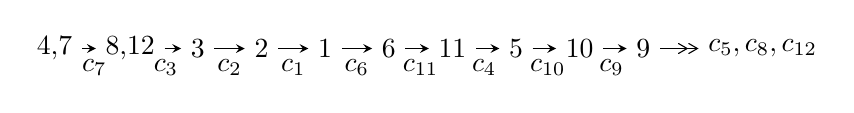
\begin{tikzpicture}[x=23pt, y=7pt]
	% node
	\node (A0) at (-1/8, 0) {4,7};
	\node (A1) at (17/16, 0) {8,12};
	\node (A2) at (17/8, 0) {3};
	\node (A3) at (25/8, 0) {2};
	\node (A4) at (33/8, 0) {1};
	\node (A5) at (41/8, 0) {6};
	\node (A6) at (49/8, 0) {11};
	\node (A7) at (57/8, 0) {5};
	\node (A8) at (65/8, 0) {10};
	\node (A9) at (73/8, 0) {9};
	\node (C1) at (1/2, -1) {$c_{7}$};
	\node (C2) at (13/8, -1) {$c_{3}$};
	\node (C3) at (21/8, -1) {$c_{2}$};
	\node (C4) at (29/8, -1) {$c_{1}$};
	\node (C5) at (37/8, -1) {$c_{6}$};
	\node (C6) at (45/8, -1) {$c_{11}$};
	\node (C7) at (53/8, -1) {$c_{4}$};
	\node (C8) at (61/8, -1) {$c_{10}$};
	\node (C9) at (69/8, -1) {$c_{9}$};
	\node (A10) at (11, 0) {$c_{5},c_{8},c_{12}$};

	% edge
	\draw[->,>=stealth]	
	(A0) edge (A1) (A1) edge (A2) (A2) edge (A3) (A3) edge (A4) (A4) edge (A5) (A5) edge (A6) (A6) edge (A7) (A7) edge (A8) (A8) edge (A9) ;
	\draw[->>,>={angle 60}]	
	(A9) edge (A10);
\end{tikzpicture} \\ 

\end{tabular} \\

\footnotetext{
The image of knot diagram is generated by the software ``\textbf{Draw programme}" developed by Andrew Bartholomew(\url{http://www.layer8.co.uk/maths/draw/index.htm\#Running-draw}), where we modified some parts for our purpose(\url{https://github.com/CATsTAILs/LinksPainter}).
}\phantom \\ \newline 
\centering \textbf{Ideals for irreducible components\footnotemark of $X_{\text{par}}$} 
 
\begin{align*}
I^u_{1}&=\langle 
-1.27157\times10^{201} u^{63}+4.53753\times10^{202} u^{62}+\cdots+4.88020\times10^{203} b+5.65168\times10^{203},\\
\phantom{I^u_{1}}&\phantom{= \langle  }-8.48877\times10^{202} u^{63}+3.19137\times10^{203} u^{62}+\cdots+4.88020\times10^{203} a+4.32696\times10^{204},\\
\phantom{I^u_{1}}&\phantom{= \langle  }u^{64}-3 u^{63}+\cdots+9 u+1\rangle \\
I^u_{2}&=\langle 
11150600999535 u^{21}-14783938671492 u^{20}+\cdots+6959144640989 b+6978556189620,\\
\phantom{I^u_{2}}&\phantom{= \langle  }68211367039889 u^{21}-98301657351572 u^{20}+\cdots+6959144640989 a+42747854441200,\\
\phantom{I^u_{2}}&\phantom{= \langle  }u^{22}-2 u^{21}+\cdots-2 u+1\rangle \\
\\
\end{align*}
\raggedright * 2 irreducible components of $\dim_{\mathbb{C}}=0$, with total 86 representations.\\
\footnotetext{All coefficients of polynomials are rational numbers. But the coefficients are sometimes approximated in decimal forms when there is not enough margin.}
\newpage
\renewcommand{\arraystretch}{1}
\centering \section*{I. $I^u_{1}= \langle -1.27\times10^{201} u^{63}+4.54\times10^{202} u^{62}+\cdots+4.88\times10^{203} b+5.65\times10^{203},\;-8.49\times10^{202} u^{63}+3.19\times10^{203} u^{62}+\cdots+4.88\times10^{203} a+4.33\times10^{204},\;u^{64}-3 u^{63}+\cdots+9 u+1 \rangle$}
\flushleft \textbf{(i) Arc colorings}\\
\begin{tabular}{m{7pt} m{180pt} m{7pt} m{180pt} }
\flushright $a_{4}=$&$\begin{pmatrix}0\\u\end{pmatrix}$ \\
\flushright $a_{7}=$&$\begin{pmatrix}1\\0\end{pmatrix}$ \\
\flushright $a_{8}=$&$\begin{pmatrix}1\\u^2\end{pmatrix}$ \\
\flushright $a_{12}=$&$\begin{pmatrix}0.173943 u^{63}-0.653942 u^{62}+\cdots-7.97727 u-8.86637\\0.00260557 u^{63}-0.0929784 u^{62}+\cdots-5.15924 u-1.15808\end{pmatrix}$ \\
\flushright $a_{3}=$&$\begin{pmatrix}2.45092 u^{63}-7.73517 u^{62}+\cdots+96.0329 u+1.67519\\0.298291 u^{63}-0.938637 u^{62}+\cdots+8.62009 u+0.0738241\end{pmatrix}$ \\
\flushright $a_{2}=$&$\begin{pmatrix}2.74921 u^{63}-8.67381 u^{62}+\cdots+104.653 u+1.74901\\0.298291 u^{63}-0.938637 u^{62}+\cdots+8.62009 u+0.0738241\end{pmatrix}$ \\
\flushright $a_{1}=$&$\begin{pmatrix}-0.785214 u^{63}+2.30228 u^{62}+\cdots-45.6518 u-11.3768\\0.0982812 u^{63}-0.446815 u^{62}+\cdots-4.70790 u-0.845415\end{pmatrix}$ \\
\flushright $a_{6}=$&$\begin{pmatrix}2.72840 u^{63}-8.38407 u^{62}+\cdots+128.985 u+8.01125\\0.206745 u^{63}-0.717715 u^{62}+\cdots+6.00433 u-0.407776\end{pmatrix}$ \\
\flushright $a_{11}=$&$\begin{pmatrix}0.190318 u^{63}-0.794890 u^{62}+\cdots-14.1516 u-10.1566\\0.0430267 u^{63}-0.228287 u^{62}+\cdots-4.34921 u-1.06626\end{pmatrix}$ \\
\flushright $a_{5}=$&$\begin{pmatrix}2.91738 u^{63}-9.20280 u^{62}+\cdots+106.391 u+0.595014\\0.172195 u^{63}-0.530154 u^{62}+\cdots+5.86731 u-0.320917\end{pmatrix}$ \\
\flushright $a_{10}=$&$\begin{pmatrix}0.147291 u^{63}-0.566603 u^{62}+\cdots-9.80237 u-9.09030\\0.0430267 u^{63}-0.228287 u^{62}+\cdots-4.34921 u-1.06626\end{pmatrix}$ \\
\flushright $a_{9}=$&$\begin{pmatrix}4.19462 u^{63}-13.2279 u^{62}+\cdots+159.234 u+3.94471\\0.430364 u^{63}-1.40465 u^{62}+\cdots+11.1768 u-0.195577\end{pmatrix}$\\&\end{tabular}
\flushleft \textbf{(ii) Obstruction class $= -1$}\\~\\
\flushleft \textbf{(iii) Cusp Shapes $= -0.166269 u^{63}+0.633459 u^{62}+\cdots-0.558660 u-1.79988$}\\~\\
\newpage\renewcommand{\arraystretch}{1}
\flushleft \textbf{(iv) u-Polynomials at the component}\newline \\
\begin{tabular}{m{50pt}|m{274pt}}
Crossings & \hspace{64pt}u-Polynomials at each crossing \\
\hline $$\begin{aligned}c_{1}\end{aligned}$$&$\begin{aligned}
&u^{64}+81 u^{63}+\cdots+20217 u+961
\end{aligned}$\\
\hline $$\begin{aligned}c_{2},c_{6}\end{aligned}$$&$\begin{aligned}
&u^{64}- u^{63}+\cdots-335 u+31
\end{aligned}$\\
\hline $$\begin{aligned}c_{3}\end{aligned}$$&$\begin{aligned}
&u^{64}-5 u^{63}+\cdots-649 u+91
\end{aligned}$\\
\hline $$\begin{aligned}c_{4}\end{aligned}$$&$\begin{aligned}
&u^{64}- u^{62}+\cdots+22 u+1
\end{aligned}$\\
\hline $$\begin{aligned}c_{5},c_{8}\end{aligned}$$&$\begin{aligned}
&u^{64}- u^{63}+\cdots+184 u+68
\end{aligned}$\\
\hline $$\begin{aligned}c_{7}\end{aligned}$$&$\begin{aligned}
&u^{64}+3 u^{63}+\cdots-9 u+1
\end{aligned}$\\
\hline $$\begin{aligned}c_{9}\end{aligned}$$&$\begin{aligned}
&u^{64}+46 u^{62}+\cdots-120919 u+79381
\end{aligned}$\\
\hline $$\begin{aligned}c_{10}\end{aligned}$$&$\begin{aligned}
&u^{64}- u^{63}+\cdots-4829 u+811
\end{aligned}$\\
\hline $$\begin{aligned}c_{11}\end{aligned}$$&$\begin{aligned}
&u^{64}+5 u^{63}+\cdots-399 u+73
\end{aligned}$\\
\hline $$\begin{aligned}c_{12}\end{aligned}$$&$\begin{aligned}
&u^{64}-4 u^{63}+\cdots-163376 u+24613
\end{aligned}$\\
\hline
\end{tabular}\\~\\
\newpage\renewcommand{\arraystretch}{1}
\flushleft \textbf{(v) Riley Polynomials at the component}\newline \\
\begin{tabular}{m{50pt}|m{274pt}}
Crossings & \hspace{64pt}Riley Polynomials at each crossing \\
\hline $$\begin{aligned}c_{1}\end{aligned}$$&$\begin{aligned}
&y^{64}-185 y^{63}+\cdots-197253273 y+923521
\end{aligned}$\\
\hline $$\begin{aligned}c_{2},c_{6}\end{aligned}$$&$\begin{aligned}
&y^{64}-81 y^{63}+\cdots-20217 y+961
\end{aligned}$\\
\hline $$\begin{aligned}c_{3}\end{aligned}$$&$\begin{aligned}
&y^{64}+33 y^{63}+\cdots+282593 y+8281
\end{aligned}$\\
\hline $$\begin{aligned}c_{4}\end{aligned}$$&$\begin{aligned}
&y^{64}-2 y^{63}+\cdots-40 y+1
\end{aligned}$\\
\hline $$\begin{aligned}c_{5},c_{8}\end{aligned}$$&$\begin{aligned}
&y^{64}-35 y^{63}+\cdots-314288 y+4624
\end{aligned}$\\
\hline $$\begin{aligned}c_{7}\end{aligned}$$&$\begin{aligned}
&y^{64}- y^{63}+\cdots+35 y+1
\end{aligned}$\\
\hline $$\begin{aligned}c_{9}\end{aligned}$$&$\begin{aligned}
&y^{64}+92 y^{63}+\cdots+301309418769 y+6301343161
\end{aligned}$\\
\hline $$\begin{aligned}c_{10}\end{aligned}$$&$\begin{aligned}
&y^{64}+19 y^{63}+\cdots+39598139 y+657721
\end{aligned}$\\
\hline $$\begin{aligned}c_{11}\end{aligned}$$&$\begin{aligned}
&y^{64}+19 y^{63}+\cdots+133529 y+5329
\end{aligned}$\\
\hline $$\begin{aligned}c_{12}\end{aligned}$$&$\begin{aligned}
&y^{64}+78 y^{63}+\cdots+15272118522 y+605799769
\end{aligned}$\\
\hline
\end{tabular}\\~\\
\newpage\flushleft \textbf{(vi) Complex Volumes and Cusp Shapes}
$$\begin{array}{c|c|c}  
\text{Solutions to }I^u_{1}& \I (\text{vol} + \sqrt{-1}CS) & \text{Cusp shape}\\
 \hline 
\begin{aligned}
u &= -0.313536 + 0.928430 I \\
a &= \phantom{-}1.72819 + 0.46093 I \\
b &= -1.146680 - 0.590328 I\end{aligned}
 & -4.60431 + 6.37966 I & \phantom{-}4.21851 - 5.44879 I \\ \hline\begin{aligned}
u &= -0.313536 - 0.928430 I \\
a &= \phantom{-}1.72819 - 0.46093 I \\
b &= -1.146680 + 0.590328 I\end{aligned}
 & -4.60431 - 6.37966 I & \phantom{-}4.21851 + 5.44879 I \\ \hline\begin{aligned}
u &= \phantom{-}0.795119 + 0.560822 I \\
a &= -1.17974 + 1.14518 I \\
b &= -0.549493 + 0.075343 I\end{aligned}
 & -8.95792 - 7.99927 I & -2.45661 + 6.71553 I \\ \hline\begin{aligned}
u &= \phantom{-}0.795119 - 0.560822 I \\
a &= -1.17974 - 1.14518 I \\
b &= -0.549493 - 0.075343 I\end{aligned}
 & -8.95792 + 7.99927 I & -2.45661 - 6.71553 I \\ \hline\begin{aligned}
u &= \phantom{-}0.547034 + 0.887218 I \\
a &= -1.47486 + 0.31618 I \\
b &= \phantom{-}1.240990 - 0.613531 I\end{aligned}
 & -5.34471 - 2.73153 I & \phantom{-}1.11554 + 3.31035 I \\ \hline\begin{aligned}
u &= \phantom{-}0.547034 - 0.887218 I \\
a &= -1.47486 - 0.31618 I \\
b &= \phantom{-}1.240990 + 0.613531 I\end{aligned}
 & -5.34471 + 2.73153 I & \phantom{-}1.11554 - 3.31035 I \\ \hline\begin{aligned}
u &= \phantom{-}0.905830 + 0.202592 I \\
a &= \phantom{-}0.801451 - 0.189428 I \\
b &= \phantom{-}0.0992545 - 0.0572400 I\end{aligned}
 & -1.89160 - 0.13655 I & -5.74382 - 0.58160 I \\ \hline\begin{aligned}
u &= \phantom{-}0.905830 - 0.202592 I \\
a &= \phantom{-}0.801451 + 0.189428 I \\
b &= \phantom{-}0.0992545 + 0.0572400 I\end{aligned}
 & -1.89160 + 0.13655 I & -5.74382 + 0.58160 I \\ \hline\begin{aligned}
u &= -0.718433 + 0.579587 I \\
a &= -1.138640 - 0.604435 I \\
b &= \phantom{-}0.168043 + 0.042894 I\end{aligned}
 & -1.66794 + 4.14809 I & -1.94761 - 7.92865 I \\ \hline\begin{aligned}
u &= -0.718433 - 0.579587 I \\
a &= -1.138640 + 0.604435 I \\
b &= \phantom{-}0.168043 - 0.042894 I\end{aligned}
 & -1.66794 - 4.14809 I & -1.94761 + 7.92865 I\\
 \hline 
 \end{array}$$\newpage$$\begin{array}{c|c|c}  
\text{Solutions to }I^u_{1}& \I (\text{vol} + \sqrt{-1}CS) & \text{Cusp shape}\\
 \hline 
\begin{aligned}
u &= \phantom{-}0.931771 + 0.606631 I \\
a &= \phantom{-}0.767324 + 0.472502 I \\
b &= -0.903443 - 0.525413 I\end{aligned}
 & \phantom{-}3.11129 - 4.90246 I & \phantom{-0.000000 -}0. + 6.64058 I \\ \hline\begin{aligned}
u &= \phantom{-}0.931771 - 0.606631 I \\
a &= \phantom{-}0.767324 - 0.472502 I \\
b &= -0.903443 + 0.525413 I\end{aligned}
 & \phantom{-}3.11129 + 4.90246 I & \phantom{-0.000000 } 0. - 6.64058 I \\ \hline\begin{aligned}
u &= \phantom{-}0.608117 + 0.645945 I \\
a &= \phantom{-}1.54613 + 0.89155 I \\
b &= -0.966015 + 0.576493 I\end{aligned}
 & \phantom{-}3.28606 - 3.38738 I & \phantom{-}3.49350 + 7.72062 I \\ \hline\begin{aligned}
u &= \phantom{-}0.608117 - 0.645945 I \\
a &= \phantom{-}1.54613 - 0.89155 I \\
b &= -0.966015 - 0.576493 I\end{aligned}
 & \phantom{-}3.28606 + 3.38738 I & \phantom{-}3.49350 - 7.72062 I \\ \hline\begin{aligned}
u &= \phantom{-}1.118670 + 0.262763 I \\
a &= -0.425297 + 0.859369 I \\
b &= -0.264219 - 0.462135 I\end{aligned}
 & -7.70013 - 1.88690 I & \phantom{-0.000000 } 0 \\ \hline\begin{aligned}
u &= \phantom{-}1.118670 - 0.262763 I \\
a &= -0.425297 - 0.859369 I \\
b &= -0.264219 + 0.462135 I\end{aligned}
 & -7.70013 + 1.88690 I & \phantom{-0.000000 } 0 \\ \hline\begin{aligned}
u &= \phantom{-}0.415838 + 0.711049 I \\
a &= -0.21037 - 1.74652 I \\
b &= \phantom{-}0.843215 - 0.109604 I\end{aligned}
 & \phantom{-}0.231680 - 1.139720 I & \phantom{-}4.34801 + 7.52749 I \\ \hline\begin{aligned}
u &= \phantom{-}0.415838 - 0.711049 I \\
a &= -0.21037 + 1.74652 I \\
b &= \phantom{-}0.843215 + 0.109604 I\end{aligned}
 & \phantom{-}0.231680 + 1.139720 I & \phantom{-}4.34801 - 7.52749 I \\ \hline\begin{aligned}
u &= -0.056636 + 0.733680 I \\
a &= -1.29377 + 1.19577 I \\
b &= \phantom{-}0.524020 + 0.229386 I\end{aligned}
 & \phantom{-}5.23978 + 1.80222 I & \phantom{-}13.43627 - 2.54767 I \\ \hline\begin{aligned}
u &= -0.056636 - 0.733680 I \\
a &= -1.29377 - 1.19577 I \\
b &= \phantom{-}0.524020 - 0.229386 I\end{aligned}
 & \phantom{-}5.23978 - 1.80222 I & \phantom{-}13.43627 + 2.54767 I\\
 \hline 
 \end{array}$$\newpage$$\begin{array}{c|c|c}  
\text{Solutions to }I^u_{1}& \I (\text{vol} + \sqrt{-1}CS) & \text{Cusp shape}\\
 \hline 
\begin{aligned}
u &= -0.667566 + 0.309584 I \\
a &= -1.32046 + 0.68489 I \\
b &= \phantom{-}0.903912 - 0.216297 I\end{aligned}
 & -0.79116 + 2.64492 I & -4.65254 + 4.03443 I \\ \hline\begin{aligned}
u &= -0.667566 - 0.309584 I \\
a &= -1.32046 - 0.68489 I \\
b &= \phantom{-}0.903912 + 0.216297 I\end{aligned}
 & -0.79116 - 2.64492 I & -4.65254 - 4.03443 I \\ \hline\begin{aligned}
u &= \phantom{-}0.142284 + 0.713386 I \\
a &= \phantom{-}1.025040 + 0.094527 I \\
b &= -1.13010 + 1.00771 I\end{aligned}
 & \phantom{-}1.51636 - 1.64164 I & \phantom{-}2.99307 + 5.98952 I \\ \hline\begin{aligned}
u &= \phantom{-}0.142284 - 0.713386 I \\
a &= \phantom{-}1.025040 - 0.094527 I \\
b &= -1.13010 - 1.00771 I\end{aligned}
 & \phantom{-}1.51636 + 1.64164 I & \phantom{-}2.99307 - 5.98952 I \\ \hline\begin{aligned}
u &= -1.172400 + 0.565699 I \\
a &= \phantom{-}0.586710 + 0.572071 I \\
b &= \phantom{-}0.708917 + 0.272244 I\end{aligned}
 & -12.35140 + 1.42793 I & \phantom{-0.000000 } 0 \\ \hline\begin{aligned}
u &= -1.172400 - 0.565699 I \\
a &= \phantom{-}0.586710 - 0.572071 I \\
b &= \phantom{-}0.708917 - 0.272244 I\end{aligned}
 & -12.35140 - 1.42793 I & \phantom{-0.000000 } 0 \\ \hline\begin{aligned}
u &= -1.335590 + 0.249330 I \\
a &= \phantom{-}0.055887 + 0.659381 I \\
b &= \phantom{-}0.436791 - 0.571046 I\end{aligned}
 & -8.51911 - 1.79325 I & \phantom{-0.000000 } 0 \\ \hline\begin{aligned}
u &= -1.335590 - 0.249330 I \\
a &= \phantom{-}0.055887 - 0.659381 I \\
b &= \phantom{-}0.436791 + 0.571046 I\end{aligned}
 & -8.51911 + 1.79325 I & \phantom{-0.000000 } 0 \\ \hline\begin{aligned}
u &= \phantom{-}1.036250 + 0.894606 I \\
a &= -0.641417 - 0.592734 I \\
b &= \phantom{-}1.56427 + 0.08327 I\end{aligned}
 & \phantom{-}3.05175 - 2.56289 I & \phantom{-0.000000 } 0 \\ \hline\begin{aligned}
u &= \phantom{-}1.036250 - 0.894606 I \\
a &= -0.641417 + 0.592734 I \\
b &= \phantom{-}1.56427 - 0.08327 I\end{aligned}
 & \phantom{-}3.05175 + 2.56289 I & \phantom{-0.000000 } 0\\
 \hline 
 \end{array}$$\newpage$$\begin{array}{c|c|c}  
\text{Solutions to }I^u_{1}& \I (\text{vol} + \sqrt{-1}CS) & \text{Cusp shape}\\
 \hline 
\begin{aligned}
u &= \phantom{-}0.201469 + 0.595721 I \\
a &= \phantom{-}0.141582 + 0.261679 I \\
b &= \phantom{-}0.368885 + 0.672035 I\end{aligned}
 & \phantom{-}0.180822 - 1.357760 I & \phantom{-}1.47757 + 4.14647 I \\ \hline\begin{aligned}
u &= \phantom{-}0.201469 - 0.595721 I \\
a &= \phantom{-}0.141582 - 0.261679 I \\
b &= \phantom{-}0.368885 - 0.672035 I\end{aligned}
 & \phantom{-}0.180822 + 1.357760 I & \phantom{-}1.47757 - 4.14647 I \\ \hline\begin{aligned}
u &= -0.057818 + 1.371080 I \\
a &= -0.545883 + 0.246577 I \\
b &= \phantom{-}2.01305 - 1.25534 I\end{aligned}
 & -5.83121 + 3.82325 I & \phantom{-0.000000 } 0 \\ \hline\begin{aligned}
u &= -0.057818 - 1.371080 I \\
a &= -0.545883 - 0.246577 I \\
b &= \phantom{-}2.01305 + 1.25534 I\end{aligned}
 & -5.83121 - 3.82325 I & \phantom{-0.000000 } 0 \\ \hline\begin{aligned}
u &= \phantom{-}0.498905 + 0.371242 I \\
a &= -1.65967 - 0.53182 I \\
b &= \phantom{-}1.75112 - 1.24099 I\end{aligned}
 & -7.58122 - 7.03725 I & -3.47625 + 8.84937 I \\ \hline\begin{aligned}
u &= \phantom{-}0.498905 - 0.371242 I \\
a &= -1.65967 + 0.53182 I \\
b &= \phantom{-}1.75112 + 1.24099 I\end{aligned}
 & -7.58122 + 7.03725 I & -3.47625 - 8.84937 I \\ \hline\begin{aligned}
u &= -0.90400 + 1.09021 I \\
a &= \phantom{-}0.794373 - 0.155195 I \\
b &= -1.40953 - 0.23797 I\end{aligned}
 & \phantom{-}5.85881 + 7.03857 I & \phantom{-0.000000 } 0 \\ \hline\begin{aligned}
u &= -0.90400 - 1.09021 I \\
a &= \phantom{-}0.794373 + 0.155195 I \\
b &= -1.40953 + 0.23797 I\end{aligned}
 & \phantom{-}5.85881 - 7.03857 I & \phantom{-0.000000 } 0 \\ \hline\begin{aligned}
u &= -0.427356 + 0.281403 I \\
a &= \phantom{-}0.219577 - 0.759859 I \\
b &= -1.255080 - 0.297545 I\end{aligned}
 & \phantom{-}2.64087 + 0.13449 I & \phantom{-}3.50237 + 3.05615 I \\ \hline\begin{aligned}
u &= -0.427356 - 0.281403 I \\
a &= \phantom{-}0.219577 + 0.759859 I \\
b &= -1.255080 + 0.297545 I\end{aligned}
 & \phantom{-}2.64087 - 0.13449 I & \phantom{-}3.50237 - 3.05615 I\\
 \hline 
 \end{array}$$\newpage$$\begin{array}{c|c|c}  
\text{Solutions to }I^u_{1}& \I (\text{vol} + \sqrt{-1}CS) & \text{Cusp shape}\\
 \hline 
\begin{aligned}
u &= -1.09532 + 1.03428 I \\
a &= -0.881703 + 0.452299 I \\
b &= \phantom{-}1.80167 + 0.70128 I\end{aligned}
 & \phantom{-}3.35796 + 9.86267 I & \phantom{-0.000000 } 0 \\ \hline\begin{aligned}
u &= -1.09532 - 1.03428 I \\
a &= -0.881703 - 0.452299 I \\
b &= \phantom{-}1.80167 - 0.70128 I\end{aligned}
 & \phantom{-}3.35796 - 9.86267 I & \phantom{-0.000000 } 0 \\ \hline\begin{aligned}
u &= -0.295497 + 0.344433 I \\
a &= \phantom{-}2.19362 - 0.77590 I \\
b &= -1.00229 - 1.72181 I\end{aligned}
 & -7.87777 + 0.76027 I & -0.44254 - 2.24356 I \\ \hline\begin{aligned}
u &= -0.295497 - 0.344433 I \\
a &= \phantom{-}2.19362 + 0.77590 I \\
b &= -1.00229 + 1.72181 I\end{aligned}
 & -7.87777 - 0.76027 I & -0.44254 + 2.24356 I \\ \hline\begin{aligned}
u &= \phantom{-}0.97455 + 1.25530 I \\
a &= \phantom{-}0.815863 + 0.115800 I \\
b &= -1.59645 + 0.91699 I\end{aligned}
 & \phantom{-}1.89181 - 7.52039 I & \phantom{-0.000000 } 0 \\ \hline\begin{aligned}
u &= \phantom{-}0.97455 - 1.25530 I \\
a &= \phantom{-}0.815863 - 0.115800 I \\
b &= -1.59645 - 0.91699 I\end{aligned}
 & \phantom{-}1.89181 + 7.52039 I & \phantom{-0.000000 } 0 \\ \hline\begin{aligned}
u &= -0.99150 + 1.25611 I \\
a &= \phantom{-}0.556030 - 0.517387 I \\
b &= -1.77104 - 0.38113 I\end{aligned}
 & \phantom{-}3.78777 - 1.85763 I & \phantom{-0.000000 } 0 \\ \hline\begin{aligned}
u &= -0.99150 - 1.25611 I \\
a &= \phantom{-}0.556030 + 0.517387 I \\
b &= -1.77104 + 0.38113 I\end{aligned}
 & \phantom{-}3.78777 + 1.85763 I & \phantom{-0.000000 } 0 \\ \hline\begin{aligned}
u &= -0.314719 + 0.204304 I \\
a &= -2.39055 + 1.35572 I \\
b &= \phantom{-}1.139280 + 0.269051 I\end{aligned}
 & -0.56044 + 2.14518 I & -4.65679 - 4.01006 I \\ \hline\begin{aligned}
u &= -0.314719 - 0.204304 I \\
a &= -2.39055 - 1.35572 I \\
b &= \phantom{-}1.139280 - 0.269051 I\end{aligned}
 & -0.56044 - 2.14518 I & -4.65679 + 4.01006 I\\
 \hline 
 \end{array}$$\newpage$$\begin{array}{c|c|c}  
\text{Solutions to }I^u_{1}& \I (\text{vol} + \sqrt{-1}CS) & \text{Cusp shape}\\
 \hline 
\begin{aligned}
u &= \phantom{-}1.15220 + 1.15374 I \\
a &= -0.933219 - 0.281370 I \\
b &= \phantom{-}1.70870 - 1.18039 I\end{aligned}
 & -5.2447 - 15.7535 I & \phantom{-0.000000 } 0 \\ \hline\begin{aligned}
u &= \phantom{-}1.15220 - 1.15374 I \\
a &= -0.933219 + 0.281370 I \\
b &= \phantom{-}1.70870 + 1.18039 I\end{aligned}
 & -5.2447 + 15.7535 I & \phantom{-0.000000 } 0 \\ \hline\begin{aligned}
u &= \phantom{-}0.93576 + 1.41846 I \\
a &= -0.435534 - 0.232731 I \\
b &= \phantom{-}1.57902 - 0.12336 I\end{aligned}
 & \phantom{-}1.47439 - 1.95616 I & \phantom{-0.000000 } 0 \\ \hline\begin{aligned}
u &= \phantom{-}0.93576 - 1.41846 I \\
a &= -0.435534 + 0.232731 I \\
b &= \phantom{-}1.57902 + 0.12336 I\end{aligned}
 & \phantom{-}1.47439 + 1.95616 I & \phantom{-0.000000 } 0 \\ \hline\begin{aligned}
u &= \phantom{-}1.30479 + 1.13160 I \\
a &= \phantom{-}0.634730 + 0.483139 I \\
b &= -1.69635 + 1.46152 I\end{aligned}
 & \phantom{-}2.53445 - 3.97108 I & \phantom{-0.000000 } 0 \\ \hline\begin{aligned}
u &= \phantom{-}1.30479 - 1.13160 I \\
a &= \phantom{-}0.634730 - 0.483139 I \\
b &= -1.69635 - 1.46152 I\end{aligned}
 & \phantom{-}2.53445 + 3.97108 I & \phantom{-0.000000 } 0 \\ \hline\begin{aligned}
u &= -1.64567 + 0.75087 I \\
a &= -0.318200 + 0.497722 I \\
b &= \phantom{-}0.506486 + 1.315920 I\end{aligned}
 & \phantom{-}4.34227 + 0.36034 I & \phantom{-0.000000 } 0 \\ \hline\begin{aligned}
u &= -1.64567 - 0.75087 I \\
a &= -0.318200 - 0.497722 I \\
b &= \phantom{-}0.506486 - 1.315920 I\end{aligned}
 & \phantom{-}4.34227 - 0.36034 I & \phantom{-0.000000 } 0 \\ \hline\begin{aligned}
u &= -1.21980 + 1.35210 I \\
a &= \phantom{-}0.721956 - 0.216760 I \\
b &= -1.86466 - 1.57937 I\end{aligned}
 & -9.44086 + 7.17279 I & \phantom{-0.000000 } 0 \\ \hline\begin{aligned}
u &= -1.21980 - 1.35210 I \\
a &= \phantom{-}0.721956 + 0.216760 I \\
b &= -1.86466 + 1.57937 I\end{aligned}
 & -9.44086 - 7.17279 I & \phantom{-0.000000 } 0\\
 \hline 
 \end{array}$$\newpage$$\begin{array}{c|c|c}  
\text{Solutions to }I^u_{1}& \I (\text{vol} + \sqrt{-1}CS) & \text{Cusp shape}\\
 \hline 
\begin{aligned}
u &= -0.082568 + 0.145421 I \\
a &= -8.02990 - 1.39710 I \\
b &= -0.508076 - 0.441255 I\end{aligned}
 & \phantom{-}3.14263 - 0.58927 I & -2.43518 - 0.70079 I \\ \hline\begin{aligned}
u &= -0.082568 - 0.145421 I \\
a &= -8.02990 + 1.39710 I \\
b &= -0.508076 + 0.441255 I\end{aligned}
 & \phantom{-}3.14263 + 0.58927 I & -2.43518 + 0.70079 I \\ \hline\begin{aligned}
u &= \phantom{-}1.22982 + 1.54138 I \\
a &= \phantom{-}0.290748 + 0.445396 I \\
b &= -1.79422 + 0.03950 I\end{aligned}
 & -4.98726 + 6.57805 I & \phantom{-0.000000 } 0 \\ \hline\begin{aligned}
u &= \phantom{-}1.22982 - 1.54138 I \\
a &= \phantom{-}0.290748 - 0.445396 I \\
b &= -1.79422 - 0.03950 I\end{aligned}
 & -4.98726 - 6.57805 I & \phantom{-0.000000 } 0\\
 \hline 
 \end{array}$$\newpage\newpage\renewcommand{\arraystretch}{1}
\centering \section*{II. $I^u_{2}= \langle 1.12\times10^{13} u^{21}-1.48\times10^{13} u^{20}+\cdots+6.96\times10^{12} b+6.98\times10^{12},\;6.82\times10^{13} u^{21}-9.83\times10^{13} u^{20}+\cdots+6.96\times10^{12} a+4.27\times10^{13},\;u^{22}-2 u^{21}+\cdots-2 u+1 \rangle$}
\flushleft \textbf{(i) Arc colorings}\\
\begin{tabular}{m{7pt} m{180pt} m{7pt} m{180pt} }
\flushright $a_{4}=$&$\begin{pmatrix}0\\u\end{pmatrix}$ \\
\flushright $a_{7}=$&$\begin{pmatrix}1\\0\end{pmatrix}$ \\
\flushright $a_{8}=$&$\begin{pmatrix}1\\u^2\end{pmatrix}$ \\
\flushright $a_{12}=$&$\begin{pmatrix}-9.80169 u^{21}+14.1255 u^{20}+\cdots-29.4692 u-6.14269\\-1.60229 u^{21}+2.12439 u^{20}+\cdots-2.19395 u-1.00279\end{pmatrix}$ \\
\flushright $a_{3}=$&$\begin{pmatrix}2.23984 u^{21}-19.7513 u^{20}+\cdots+45.8986 u-51.8152\\-0.923468 u^{21}+2.06927 u^{20}+\cdots-4.08774 u+2.55849\end{pmatrix}$ \\
\flushright $a_{2}=$&$\begin{pmatrix}1.31637 u^{21}-17.6820 u^{20}+\cdots+41.8109 u-49.2567\\-0.923468 u^{21}+2.06927 u^{20}+\cdots-4.08774 u+2.55849\end{pmatrix}$ \\
\flushright $a_{1}=$&$\begin{pmatrix}-11.7551 u^{21}+19.2178 u^{20}+\cdots-36.0736 u+1.44016\\1.38030 u^{21}-2.46786 u^{20}+\cdots+4.94250 u-0.529976\end{pmatrix}$ \\
\flushright $a_{6}=$&$\begin{pmatrix}-6.56215 u^{21}+26.1647 u^{20}+\cdots-57.6907 u+50.1938\\1.59529 u^{21}-3.25044 u^{20}+\cdots+7.14956 u-3.05913\end{pmatrix}$ \\
\flushright $a_{11}=$&$\begin{pmatrix}-11.9938 u^{21}+15.5512 u^{20}+\cdots-30.5092 u-12.6233\\-1.86680 u^{21}+3.47738 u^{20}+\cdots-5.91910 u+1.95585\end{pmatrix}$ \\
\flushright $a_{5}=$&$\begin{pmatrix}15.6209 u^{21}-49.7963 u^{20}+\cdots+106.240 u-77.5520\\-4.91539 u^{21}+9.58345 u^{20}+\cdots-19.0836 u+5.53084\end{pmatrix}$ \\
\flushright $a_{10}=$&$\begin{pmatrix}-10.1270 u^{21}+12.0738 u^{20}+\cdots-24.5900 u-14.5792\\-1.86680 u^{21}+3.47738 u^{20}+\cdots-5.91910 u+1.95585\end{pmatrix}$ \\
\flushright $a_{9}=$&$\begin{pmatrix}13.9617 u^{21}-40.0092 u^{20}+\cdots+77.7503 u-57.2328\\-9.01335 u^{21}+17.7162 u^{20}+\cdots-35.1771 u+10.1227\end{pmatrix}$\\&\end{tabular}
\flushleft \textbf{(ii) Obstruction class $= 1$}\\~\\
\flushleft \textbf{(iii) Cusp Shapes $= \frac{77090866342321}{6959144640989} u^{21}+\frac{24417195627111}{6959144640989} u^{20}+\cdots-\frac{131924333737762}{6959144640989} u+\frac{529449466425046}{6959144640989}$}\\~\\
\newpage\renewcommand{\arraystretch}{1}
\flushleft \textbf{(iv) u-Polynomials at the component}\newline \\
\begin{tabular}{m{50pt}|m{274pt}}
Crossings & \hspace{64pt}u-Polynomials at each crossing \\
\hline $$\begin{aligned}c_{1}\end{aligned}$$&$\begin{aligned}
&u^{22}-22 u^{21}+\cdots-18 u+1
\end{aligned}$\\
\hline $$\begin{aligned}c_{2}\end{aligned}$$&$\begin{aligned}
&u^{22}-11 u^{20}+\cdots-4 u+1
\end{aligned}$\\
\hline $$\begin{aligned}c_{3}\end{aligned}$$&$\begin{aligned}
&u^{22}+6 u^{21}+\cdots+22 u+7
\end{aligned}$\\
\hline $$\begin{aligned}c_{4}\end{aligned}$$&$\begin{aligned}
&u^{22}+3 u^{21}+\cdots-3 u+1
\end{aligned}$\\
\hline $$\begin{aligned}c_{5}\end{aligned}$$&$\begin{aligned}
&u^{22}-10 u^{20}+\cdots-4 u+4
\end{aligned}$\\
\hline $$\begin{aligned}c_{6}\end{aligned}$$&$\begin{aligned}
&u^{22}-11 u^{20}+\cdots+4 u+1
\end{aligned}$\\
\hline $$\begin{aligned}c_{7}\end{aligned}$$&$\begin{aligned}
&u^{22}-2 u^{21}+\cdots-2 u+1
\end{aligned}$\\
\hline $$\begin{aligned}c_{8}\end{aligned}$$&$\begin{aligned}
&u^{22}-10 u^{20}+\cdots+4 u+4
\end{aligned}$\\
\hline $$\begin{aligned}c_{9}\end{aligned}$$&$\begin{aligned}
&u^{22}- u^{21}+\cdots+6 u+1
\end{aligned}$\\
\hline $$\begin{aligned}c_{10}\end{aligned}$$&$\begin{aligned}
&u^{22}+2 u^{21}+\cdots+4 u+11
\end{aligned}$\\
\hline $$\begin{aligned}c_{11}\end{aligned}$$&$\begin{aligned}
&u^{22}-2 u^{21}+\cdots-2 u+1
\end{aligned}$\\
\hline $$\begin{aligned}c_{12}\end{aligned}$$&$\begin{aligned}
&u^{22}-3 u^{21}+\cdots+u+1
\end{aligned}$\\
\hline
\end{tabular}\\~\\
\newpage\renewcommand{\arraystretch}{1}
\flushleft \textbf{(v) Riley Polynomials at the component}\newline \\
\begin{tabular}{m{50pt}|m{274pt}}
Crossings & \hspace{64pt}Riley Polynomials at each crossing \\
\hline $$\begin{aligned}c_{1}\end{aligned}$$&$\begin{aligned}
&y^{22}-34 y^{21}+\cdots-86 y+1
\end{aligned}$\\
\hline $$\begin{aligned}c_{2},c_{6}\end{aligned}$$&$\begin{aligned}
&y^{22}-22 y^{21}+\cdots-18 y+1
\end{aligned}$\\
\hline $$\begin{aligned}c_{3}\end{aligned}$$&$\begin{aligned}
&y^{22}+12 y^{21}+\cdots+552 y+49
\end{aligned}$\\
\hline $$\begin{aligned}c_{4}\end{aligned}$$&$\begin{aligned}
&y^{22}-3 y^{21}+\cdots-21 y+1
\end{aligned}$\\
\hline $$\begin{aligned}c_{5},c_{8}\end{aligned}$$&$\begin{aligned}
&y^{22}-20 y^{21}+\cdots-360 y+16
\end{aligned}$\\
\hline $$\begin{aligned}c_{7}\end{aligned}$$&$\begin{aligned}
&y^{22}-2 y^{21}+\cdots+10 y+1
\end{aligned}$\\
\hline $$\begin{aligned}c_{9}\end{aligned}$$&$\begin{aligned}
&y^{22}+11 y^{21}+\cdots-8 y+1
\end{aligned}$\\
\hline $$\begin{aligned}c_{10}\end{aligned}$$&$\begin{aligned}
&y^{22}+10 y^{21}+\cdots-1930 y+121
\end{aligned}$\\
\hline $$\begin{aligned}c_{11}\end{aligned}$$&$\begin{aligned}
&y^{22}+10 y^{21}+\cdots+20 y+1
\end{aligned}$\\
\hline $$\begin{aligned}c_{12}\end{aligned}$$&$\begin{aligned}
&y^{22}+9 y^{21}+\cdots-11 y+1
\end{aligned}$\\
\hline
\end{tabular}\\~\\
\newpage\flushleft \textbf{(vi) Complex Volumes and Cusp Shapes}
$$\begin{array}{c|c|c}  
\text{Solutions to }I^u_{2}& \I (\text{vol} + \sqrt{-1}CS) & \text{Cusp shape}\\
 \hline 
\begin{aligned}
u &= -0.059740 + 0.923637 I \\
a &= -0.825379 + 0.806774 I \\
b &= \phantom{-}1.80958 - 0.44104 I\end{aligned}
 & -6.67000 - 6.08404 I & \phantom{-}0.07907 + 4.41733 I \\ \hline\begin{aligned}
u &= -0.059740 - 0.923637 I \\
a &= -0.825379 - 0.806774 I \\
b &= \phantom{-}1.80958 + 0.44104 I\end{aligned}
 & -6.67000 + 6.08404 I & \phantom{-}0.07907 - 4.41733 I \\ \hline\begin{aligned}
u &= \phantom{-}1.110170 + 0.156513 I \\
a &= -0.218712 + 0.595946 I \\
b &= -0.565963 - 0.935358 I\end{aligned}
 & -9.15907 - 0.38779 I & -3.84597 - 0.39740 I \\ \hline\begin{aligned}
u &= \phantom{-}1.110170 - 0.156513 I \\
a &= -0.218712 - 0.595946 I \\
b &= -0.565963 + 0.935358 I\end{aligned}
 & -9.15907 + 0.38779 I & -3.84597 + 0.39740 I \\ \hline\begin{aligned}
u &= -0.560586 + 0.578524 I \\
a &= -0.162842 - 1.197430 I \\
b &= -0.873727 - 0.227661 I\end{aligned}
 & -0.093894 + 0.509045 I & -2.06274 + 2.06357 I \\ \hline\begin{aligned}
u &= -0.560586 - 0.578524 I \\
a &= -0.162842 + 1.197430 I \\
b &= -0.873727 + 0.227661 I\end{aligned}
 & -0.093894 - 0.509045 I & -2.06274 - 2.06357 I \\ \hline\begin{aligned}
u &= \phantom{-}0.468082 + 0.590835 I \\
a &= \phantom{-}0.829025 + 0.241574 I \\
b &= -1.38855 + 0.85198 I\end{aligned}
 & \phantom{-}2.61073 - 0.75532 I & \phantom{-}3.73998 + 7.77562 I \\ \hline\begin{aligned}
u &= \phantom{-}0.468082 - 0.590835 I \\
a &= \phantom{-}0.829025 - 0.241574 I \\
b &= -1.38855 - 0.85198 I\end{aligned}
 & \phantom{-}2.61073 + 0.75532 I & \phantom{-}3.73998 - 7.77562 I \\ \hline\begin{aligned}
u &= -0.585432 + 0.445145 I \\
a &= -1.368150 + 0.243037 I \\
b &= \phantom{-}0.963772 - 0.376578 I\end{aligned}
 & -0.54127 + 3.01960 I & \phantom{-}5.04193 - 10.09843 I \\ \hline\begin{aligned}
u &= -0.585432 - 0.445145 I \\
a &= -1.368150 - 0.243037 I \\
b &= \phantom{-}0.963772 + 0.376578 I\end{aligned}
 & -0.54127 - 3.01960 I & \phantom{-}5.04193 + 10.09843 I\\
 \hline 
 \end{array}$$\newpage$$\begin{array}{c|c|c}  
\text{Solutions to }I^u_{2}& \I (\text{vol} + \sqrt{-1}CS) & \text{Cusp shape}\\
 \hline 
\begin{aligned}
u &= -0.990692 + 0.939676 I \\
a &= \phantom{-}0.582887 - 0.490467 I \\
b &= -1.53592 + 0.35917 I\end{aligned}
 & \phantom{-}4.32636 + 3.84430 I & \phantom{-}4.24435 - 3.41824 I \\ \hline\begin{aligned}
u &= -0.990692 - 0.939676 I \\
a &= \phantom{-}0.582887 + 0.490467 I \\
b &= -1.53592 - 0.35917 I\end{aligned}
 & \phantom{-}4.32636 - 3.84430 I & \phantom{-}4.24435 + 3.41824 I \\ \hline\begin{aligned}
u &= \phantom{-}0.95193 + 1.04804 I \\
a &= \phantom{-}0.973386 + 0.245120 I \\
b &= -1.55211 + 0.58904 I\end{aligned}
 & \phantom{-}5.52972 - 8.35084 I & \phantom{-}2.94788 + 7.36228 I \\ \hline\begin{aligned}
u &= \phantom{-}0.95193 - 1.04804 I \\
a &= \phantom{-}0.973386 - 0.245120 I \\
b &= -1.55211 - 0.58904 I\end{aligned}
 & \phantom{-}5.52972 + 8.35084 I & \phantom{-}2.94788 - 7.36228 I \\ \hline\begin{aligned}
u &= \phantom{-}0.170032 + 0.547687 I \\
a &= -2.13940 - 0.26067 I \\
b &= \phantom{-}0.485058 + 0.571865 I\end{aligned}
 & \phantom{-}4.46696 + 2.32267 I & \phantom{-}4.86381 - 5.13840 I \\ \hline\begin{aligned}
u &= \phantom{-}0.170032 - 0.547687 I \\
a &= -2.13940 + 0.26067 I \\
b &= \phantom{-}0.485058 - 0.571865 I\end{aligned}
 & \phantom{-}4.46696 - 2.32267 I & \phantom{-}4.86381 + 5.13840 I \\ \hline\begin{aligned}
u &= \phantom{-}0.208685 + 0.523085 I \\
a &= -0.89334 - 3.30383 I \\
b &= \phantom{-}0.542839 - 0.032801 I\end{aligned}
 & \phantom{-}3.64369 - 0.94557 I & \phantom{-}9.49564 + 8.08210 I \\ \hline\begin{aligned}
u &= \phantom{-}0.208685 - 0.523085 I \\
a &= -0.89334 + 3.30383 I \\
b &= \phantom{-}0.542839 + 0.032801 I\end{aligned}
 & \phantom{-}3.64369 + 0.94557 I & \phantom{-}9.49564 - 8.08210 I \\ \hline\begin{aligned}
u &= \phantom{-}1.56936 + 0.75876 I \\
a &= -0.199730 - 0.640355 I \\
b &= \phantom{-}1.07456 - 0.97330 I\end{aligned}
 & \phantom{-}4.45576 + 1.24455 I & \phantom{-}9.37100 - 3.48577 I \\ \hline\begin{aligned}
u &= \phantom{-}1.56936 - 0.75876 I \\
a &= -0.199730 + 0.640355 I \\
b &= \phantom{-}1.07456 + 0.97330 I\end{aligned}
 & \phantom{-}4.45576 - 1.24455 I & \phantom{-}9.37100 + 3.48577 I\\
 \hline 
 \end{array}$$\newpage$$\begin{array}{c|c|c}  
\text{Solutions to }I^u_{2}& \I (\text{vol} + \sqrt{-1}CS) & \text{Cusp shape}\\
 \hline 
\begin{aligned}
u &= -1.28180 + 1.51259 I \\
a &= -0.577745 + 0.315382 I \\
b &= \phantom{-}2.04046 + 1.44608 I\end{aligned}
 & \phantom{-}2.94554 + 4.02787 I & \phantom{-}13.1251 - 7.3446 I \\ \hline\begin{aligned}
u &= -1.28180 - 1.51259 I \\
a &= -0.577745 - 0.315382 I \\
b &= \phantom{-}2.04046 - 1.44608 I\end{aligned}
 & \phantom{-}2.94554 - 4.02787 I & \phantom{-}13.1251 + 7.3446 I\\
 \hline 
 \end{array}$$\newpage
\newpage\renewcommand{\arraystretch}{1}
\centering \section*{ III. u-Polynomials}
\begin{tabular}{m{50pt}|m{274pt}}
Crossings & \hspace{64pt}u-Polynomials at each crossing \\
\hline $$\begin{aligned}c_{1}\end{aligned}$$&$\begin{aligned}
&(u^{22}-22 u^{21}+\cdots-18 u+1)(u^{64}+81 u^{63}+\cdots+20217 u+961)
\end{aligned}$\\
\hline $$\begin{aligned}c_{2}\end{aligned}$$&$\begin{aligned}
&(u^{22}-11 u^{20}+\cdots-4 u+1)(u^{64}- u^{63}+\cdots-335 u+31)
\end{aligned}$\\
\hline $$\begin{aligned}c_{3}\end{aligned}$$&$\begin{aligned}
&(u^{22}+6 u^{21}+\cdots+22 u+7)(u^{64}-5 u^{63}+\cdots-649 u+91)
\end{aligned}$\\
\hline $$\begin{aligned}c_{4}\end{aligned}$$&$\begin{aligned}
&(u^{22}+3 u^{21}+\cdots-3 u+1)(u^{64}- u^{62}+\cdots+22 u+1)
\end{aligned}$\\
\hline $$\begin{aligned}c_{5}\end{aligned}$$&$\begin{aligned}
&(u^{22}-10 u^{20}+\cdots-4 u+4)(u^{64}- u^{63}+\cdots+184 u+68)
\end{aligned}$\\
\hline $$\begin{aligned}c_{6}\end{aligned}$$&$\begin{aligned}
&(u^{22}-11 u^{20}+\cdots+4 u+1)(u^{64}- u^{63}+\cdots-335 u+31)
\end{aligned}$\\
\hline $$\begin{aligned}c_{7}\end{aligned}$$&$\begin{aligned}
&(u^{22}-2 u^{21}+\cdots-2 u+1)(u^{64}+3 u^{63}+\cdots-9 u+1)
\end{aligned}$\\
\hline $$\begin{aligned}c_{8}\end{aligned}$$&$\begin{aligned}
&(u^{22}-10 u^{20}+\cdots+4 u+4)(u^{64}- u^{63}+\cdots+184 u+68)
\end{aligned}$\\
\hline $$\begin{aligned}c_{9}\end{aligned}$$&$\begin{aligned}
&(u^{22}- u^{21}+\cdots+6 u+1)(u^{64}+46 u^{62}+\cdots-120919 u+79381)
\end{aligned}$\\
\hline $$\begin{aligned}c_{10}\end{aligned}$$&$\begin{aligned}
&(u^{22}+2 u^{21}+\cdots+4 u+11)(u^{64}- u^{63}+\cdots-4829 u+811)
\end{aligned}$\\
\hline $$\begin{aligned}c_{11}\end{aligned}$$&$\begin{aligned}
&(u^{22}-2 u^{21}+\cdots-2 u+1)(u^{64}+5 u^{63}+\cdots-399 u+73)
\end{aligned}$\\
\hline $$\begin{aligned}c_{12}\end{aligned}$$&$\begin{aligned}
&(u^{22}-3 u^{21}+\cdots+u+1)(u^{64}-4 u^{63}+\cdots-163376 u+24613)
\end{aligned}$\\
\hline
\end{tabular}\newpage\renewcommand{\arraystretch}{1}
\centering \section*{ IV. Riley Polynomials}
\begin{tabular}{m{50pt}|m{274pt}}
Crossings & \hspace{64pt}Riley Polynomials at each crossing \\
\hline $$\begin{aligned}c_{1}\end{aligned}$$&$\begin{aligned}
&(y^{22}-34 y^{21}+\cdots-86 y+1)\\
&\cdot(y^{64}-185 y^{63}+\cdots-197253273 y+923521)
\end{aligned}$\\
\hline $$\begin{aligned}c_{2},c_{6}\end{aligned}$$&$\begin{aligned}
&(y^{22}-22 y^{21}+\cdots-18 y+1)(y^{64}-81 y^{63}+\cdots-20217 y+961)
\end{aligned}$\\
\hline $$\begin{aligned}c_{3}\end{aligned}$$&$\begin{aligned}
&(y^{22}+12 y^{21}+\cdots+552 y+49)(y^{64}+33 y^{63}+\cdots+282593 y+8281)
\end{aligned}$\\
\hline $$\begin{aligned}c_{4}\end{aligned}$$&$\begin{aligned}
&(y^{22}-3 y^{21}+\cdots-21 y+1)(y^{64}-2 y^{63}+\cdots-40 y+1)
\end{aligned}$\\
\hline $$\begin{aligned}c_{5},c_{8}\end{aligned}$$&$\begin{aligned}
&(y^{22}-20 y^{21}+\cdots-360 y+16)(y^{64}-35 y^{63}+\cdots-314288 y+4624)
\end{aligned}$\\
\hline $$\begin{aligned}c_{7}\end{aligned}$$&$\begin{aligned}
&(y^{22}-2 y^{21}+\cdots+10 y+1)(y^{64}- y^{63}+\cdots+35 y+1)
\end{aligned}$\\
\hline $$\begin{aligned}c_{9}\end{aligned}$$&$\begin{aligned}
&(y^{22}+11 y^{21}+\cdots-8 y+1)\\
&\cdot(y^{64}+92 y^{63}+\cdots+301309418769 y+6301343161)
\end{aligned}$\\
\hline $$\begin{aligned}c_{10}\end{aligned}$$&$\begin{aligned}
&(y^{22}+10 y^{21}+\cdots-1930 y+121)\\
&\cdot(y^{64}+19 y^{63}+\cdots+39598139 y+657721)
\end{aligned}$\\
\hline $$\begin{aligned}c_{11}\end{aligned}$$&$\begin{aligned}
&(y^{22}+10 y^{21}+\cdots+20 y+1)(y^{64}+19 y^{63}+\cdots+133529 y+5329)
\end{aligned}$\\
\hline $$\begin{aligned}c_{12}\end{aligned}$$&$\begin{aligned}
&(y^{22}+9 y^{21}+\cdots-11 y+1)\\
&\cdot(y^{64}+78 y^{63}+\cdots+15272118522 y+605799769)
\end{aligned}$\\
\hline
\end{tabular}
\vskip 2pc
\end{document}